\renewcommand{\thefootnote}{\arabic{footnote}}

\chapter[Quantum Theory of Angular Momentum and Hypergeometric series]{Quantum Theory of Angular Momentum (QTAM) and Hypergeometric series\footnote{Tribute to Dr.\ G. Ramachandran, a pioneer at the Institute of Mathematical Sciences, Madras.}}\label{chap7}

\Authorline{K. Srinivasa Rao}

\authinfo{Senior Professor (Retd.)\\ 
The Institute of Mathematical Sciences, Chennai-600113\\
\& Director (Hon.), Srinivasa Ramanujan Academy of Maths Talent.\\
(ksrao18@gmail.com)}

\section*{Preamble (biographical)}

The year was 1964, and I was a fresher from M.Sc.\ (Physics) out of Presidency College, recommended by my Professor of Physics, V. S. Angappan, as one interested in Research, to Professor Alladi Ramakrishnan, the Founder Director of the Institute of Mathematical Sciences (IMSc). I was aware, by then, that the inaugural function of IMSc was at Presidency College, on January 3, 1962, by Dr.\ S. Chandrasekhar. The first name board of the Institute was a plaque fixed to the door of the room in the new block of Presidency College, where our regular First M.Sc.\ classes were conducted, in the Forenoons and I was aware that the new Institute was allotted this room, as the starting point, until a suitable place was to the allotted by the State Government. During the next few weeks I saw Godrej bureaus appearing, and being placed to corner a portion of the room and new Physics and Mathematics books being stacked in those locked bureaus.

Two years later, on completing my final M.Sc.\ Physics six-hour practical examination successfully (which enabled me to win all the Prizes for Proficiency in Physics, for the two years 1962-'64) and relaxing for one week, I approached Professor Alladi Ramakrishnan, who after a fact finding friendly interview, offered me a Research Trainee scholarship of the Institute. He asked me not to waste time to await the results which were expected only months later but spend my time by `learning from the masters' (books). Thus was may entry into IMSc in early May 1964, based on my First Class in B.Sc. and the expectation of a First Class in M.Sc.\ (I stood first in the Exams in my batch and learned that I secured the fourth rank in the University).

By 1964, the IMSc moved into an exclusive second floor in the Central Polytechnic Building. After a few years the Founder Director was able to get for the Institute four acres of land allotted in the CIT Campus,  in the Fourth Cross street, at whose corner is the Women's Polytechnic\footnote{CIT for Central Institutes of Technology and some times also referred to as the CPT for Central Polytechnic campus -- and not the CPT-theorem!}.

The first person who took interest in me was Dr.\ G. Ramachandran (GR). I was impressed with the fact that the First MATSCIENCE (the acronym for IMSc, also the telegraphic name) Report was the Proceedings of the Kodaikanal conference convened and conducted by the dynamic Founder Director of IMSc, Professor Alladi Ramakrishnan. The second Matscience Report was entitled ``Angular Momentum", by GR. Since he was my Senior and was easily approachable in the late afternoons, I told him that I was finding his report tough to understand, he asked me to read the books on Quantum Theory of Angular Momentum (QTAM) by M. E.  Rose and A. R. Edmonds and wanted me also to explain to him, by writing on the boards (six, well-designed sliding boards in three rows of two each) what I had studied.

G. Ramachandran's papers with V. Devanathan were the ones which I was able to derive and with his help I got my foothold in the study of Pion Photoproduction from nuclei. Due to unfortunate circumstances, GR had to leave the Institute soon after my joining. He was the inspiration for my seniors V. Devanathan, K.  Ananthanarayanan, R. K. Umerjee who were all students registered with Professor Alladi Ramakrishnan.

Within a few months, A. Sundaram and R. Sridhar joined IMSc from IIT Madras, recommended by Prof.\ S. K. Srinivasan who was himself a student of Prof.\ Ramakrishnan. With the initiation into research in theoretical nuclear physics at IMSc by my seniors, GR and KA, I had the fortune of coming into contact with Dr.\ S. C. K. Nair (SCKN, 1938--1990) who was a student of Professor R. J. Blin-Stoyle of University of Sussex for his Ph.D. in $\beta$-decay of nuclei. When Nair came to know of my first paper with Anantha, SCKN said `Hey, Srinivasa Rao, see if there is any data on pion photoproduction from a closed shell nucleus, in particular $O^{16}$, in which case we are in business'.

As luck would have it, thanks to the Excellent Library, which according to the Founder Director was the heart of the Institute, I could find in the Physical Review experimental data from University of Illinois for ${}^{16}O(\gamma, \pi^+){}^{16}N$. SCKN gave me a copy of the Ph.D. Thesis (in French) of V. Gillet which contained the particle-hole wave functions for the closed shell nuclei ${}^{16}O, {}^{12}C$ and ${}^{40}Ca$. SCKN also made me learn and understand the particle-hole formalism (second quantization, synonymous with creation-annihilation operator formalism). I was thus set on my path to do research in pion photoproduction from complex nuclei for my Ph.D., with the techniques and methodology I learned from the books with the help of GR, KA and SCKN. At about that time, SCKN pointed out to me that Dr.\ Devanathan was thanked in the acknowledgment section of a paper on radiative pion capture by $^{16}O$ and this process ${}^{16}O\,(\pi^- ,\gamma)\,{}^{16}N$, being the inverse of pion photoproduction from $^{16}O$, involved the same initial and final nuclear states, and therefore, SCKN wanted me to correspond with Dr.\ Devanathan, at that time on a two-year Postdoctoral position with Prof.\ M. E. Rose, in Virginia, as he was my senior and belonged to the group of Prof.\ AR and known to me.

I still have a whole file in which I sent in my handwriting the whole of the formulation including lengthy derivations of the matrix element, and the square of the matrix element related to the cross section, using the CGLN amplitudes and the mathematical formalism developed by Ramachandran and Devanathan in a series of articles in the Nuclear Physics journal. However, in 1964, the first computer, IBM 1620, was installed in the Fundamental Engineering Research Establishment of Engineering College, Guindy, thanks to Dr.\ V. C. Kulandaiswami, who later on became the VC (Vice-Chancellor -- pun intended) of Anna University.

I did not have the computer Function sub-programs for the Clebsch-Gordan, Racah and $\ell s-jj$ transformation coefficients, essential to evaluate the cross sections for ${}^{16}O(\gamma, \pi^+){}^{16}N$ and used the Rotenberg tables for the 3-$j$ and 6-$j$ coefficients and also tables for the 9-$j$ coefficient, in a preprinted version. I could hardly debug my Fortran Program, after deriving the expression for the cross section. The details of the study of pion photoproduction are given in the article of Prof.\ Devanathan, in this volume itself and so, I am not going to dwell on that aspect here. I could not even dream of doing the numerical work on the extremely slow IBM 1620 at FERE.

And being the first to person to use the computer for the numerical work with my senior Ananathanarayanan who taught me and trained me to use the (Forgo, For-To-Go and) Fortran II on the IBM1620 at the FERE, I needed the help of Dr.\ Devanathan for the numerical work on ${}^{16}O(\gamma, \pi^+){}^{16}N$ and so sent him the entire details of the p-h formalism for the nuclear wave functions for the ground and three low-lying excited states of the final nuclear states $^{16}N(2^-,0^-,1^-,3^-)$, while $^{16}O$ was treated as the doubly magic closed shell nucleus: $(1s)^4(1p)^{12}$, with 8 protons and 8 neutrons. The comparison with the experimental data was possible only with inclusion of the Final State Interactions (FSI) of the outgoing pion with the residual final nucleus, based on the Optical Model calculations. But that required elaborate computer programming on a Fast Computer, like the CDC3600-160A computer which was available at the Tata Institute of Fundamental research, in Bombay (out of consideration for a Ph.D. student at IMSc in those days)! Therefore, a simple model was proposed to take the FSI and we called this as the Surface Production Model. In the harmonic oscillator model for the nuclear wave functions, the integrals to be evaluated were:
$$
\langle j_\ell(kr)\rangle_{n_f,\ell_f;n_i,\ell_i}\ =\  \int_c^\infty U_{n_f,\ell_f}(r)
\ j_{\ell}(kr)\ U_{n_i,\ell_i}(r)\ r^2\ dr,
$$
where the $U_{n,\ell}(r)$ refer to the harmonic oscillator wave functions for the final and initial nuclear states; $j_\ell(kr)$ is the spherical Bessel function due to the use of the plane wave approximation for $e^{i\vec{k}\cdot \vec{r}},\  \vec{k}=\vec{\mu}-\vec{\nu}$, $\vec{\mu}$ and $\vec{\nu}$ being the momenta of the initial photon and the outgoing pion, respectively. Thus, $\vec{k}$ is the momentum transferred to the nucleus. The lower limit of the integral is $c$. When this cut-off parameter, $c=0$, the integral can be evaluated analytically. And this was called as the Volume Production Model for $(\gamma,\pi)$ from complex nuclei. When $c=r_0$, one had to compute the integral numerically, using the rule
$$
\int_c^\infty f(r) dr = \int_0^\infty f(r)\ dr - \int_0^c f(r) dr
$$
so that since the first integral on the r.h.s. was known analytically for the harmonic oscillator wave functions (Gaussians), only the second of the integrals on the r.h.s had to be evaluated numerically on the computer using Simpson's Rule for numerical integration. This was referred to by our group, led by GR, as the Surface Production Model for $(\gamma,\pi)$ from nuclei. What is implied by this is that the pions released from the interior of the Nucleus of radius $R$ could be absorbed and only those not absorbed by the other nucleons would escape to be observed as outgoing pions. Thus the Surface Production Model simulates simply the FSI, and often the value of the parameter $r_0$ being related to the Radius of the Nucleus determined in electron scattering experiments by Hofstadter et.al. at Illinois, gave good fits to the energy distributions of the total cross sections for charged pion photoproduction from light nuclei.

The study of positive pion photoproduction from Oxygen-16, by V. Devanathan, K. Srinivasa Rao, S. C. K. Nair and M. Rho and its success in accounting for the energy distribution of the total cross section in the first Pion Nucleon Resonance region (320 MeV) is the first of its kind using the formalism developed by us using the p-h formalism of Gillet and the formalism in the series of papers by Ramachandran and Devanathan. This paper in the Nuclear Physics journal (Vol.\underline{B2} (1967) 329) was well received. As a sequel the author and Devanathan had a Physics Letters \underline{32B} (1970) 578) publication on the study of the effect 2p-2h correlations in the ground state wave function of $^{16}O$ on the photoproduction of positive pions $^{16}O(\gamma, \pi^+){}^{16}N$. This was followed with a study of the effect of short-range correlations in pion photoproduction from nuclei, in Can.J. Phys. \underline{53} (1975) 1292.

This author then studied charged pion photoproduction from $^{12}C$, both charged and neutral pion photoproduction of pions from this nucleus:
$$
{}^{12}C(\gamma, \pi^+){}^{12}B, \quad  {}^{12}C(\gamma, \pi^-){}^{12}N, \quad 
{}^{12}C(\gamma, \pi^0){}^{12}C.
$$

These cross sections were predicted and suggested that the negative pion photoproduction is for experimentalists to do, since the final states of ${}^{12}N$ are only two states with spin-parity $J^P=\frac{1}{2}^+$ and $\frac{1}{2}^-$. This suggestion was picked a Russian group in Dubna, from the present author's paper in the Nuclear Physics journal and on their experimental data, they superposed the energy distribution of the cross section for incident photon energies of 140 MeV to 400 MeV (around the first pion-Nucleon resonance region of 320 MeV for the incident photon) predicted by the author and stated that the Surface Production Model predictions were in agreement with the data. This was a recognition, in 1970, internationally, just when the author completed his Ph.D. thesis and one which assured him of a position in the Institute, thanks to Professor Alladi Ramakrishnan. There was no looking back after that. The author after a participation in an International Conference on Pion Photoproduction at the Rensselaer Polytechnic Institute, Troy, New York, was invited to join the experimental group which was planning an experimental studies of pion photoproduction from nuclei at the Bates Accelerator Center of the Massachusetts Institute of Technology, Boston. During the academic year 1978-1979, the author was a visiting Associate Professor at RPI, a colleague of Professor J. S. Levinger. The author was a co-guide for Professor Levinger's student, S. Malecki (Iranian), and this student successfully completed his Ph.D. thesis on pion photoproduction from nuclei.

The author had also collaborations with two other experimental\break groups -- one at the Lund Institute of Technology in Sweden led by G. G. Johnson and the paper with this group was  entitled Photproduction of $\pi^+$ from $Be^9$ (M. Nilsson on, B. Schroeder, B. Bulow, J. Grintals, G. G. Johnson, B. Lindner). The theoretical study was by the author with his Ph.D. student S. Susila (Z. für Phsyik 294A (1980) 253). The other was the group of A. M. Bernsteinat M.I.T., Boston, during the author's Visiting professorship at the Rensselaer Polytechnic Institute in Troy, New Year for the academic year (1978--79).

Since the article of Devanathan is on the formalims for $(\gamma,\pi)$ form nuclei, in this article, as my humble tribute to GR, I wish to summarize some of the significant results in the Quantum Theory of Angular Momentum, an area to which I was introduced by GR and his Matscience Report 2.

\section*{The 3-$j$ coefficient}

Consider the addition of two angular momenta:
\makeatletter
\counterwithout{equation}{chapter}
\makeatother
\begin{equation}
\vec{j_1} + \vec{j_2} = \vec{J}, \label{chap7-eq1} 
\end{equation}
whose orthonormal basis vectors are written in the Dirac bra-ket notation as:
\begin{equation} 
|j_1,m_1\rangle , |j_2,m_2\rangle, |J,M\rangle. \label{chap7-eq2}
\end{equation}

A. Clebsch and P. Gordan in their publications on the \textit{Theorie der binaren algebraischen Formen} (Tübner, Leibzig, 1872) and \textit{Uber das Formensystem binaren Formen} (Tübner, Leibzig, 1875) introduced a coefficient relating the uncoupled states to the coupled state through an orthogonal transformation:
\begin{equation}
|j_1,m_1\rangle|j_2,m_2\rangle\ =\ \sum_{J,M} C(j_1\ j_2\ J;\ m_1\ m_2\ M)\ |(j_1\ j_2)J\ M\rangle. \label{chap7-eq3}
\end{equation}

The `classical' theory of angular momentum established the existence of its inverse transformation as:
\begin{equation}
|J,M\rangle\ =\ \sum_{j_1,j_2} C(j_1\ j_2\ J;\ m_1\ m_2\ M)\ |j_1\ m_1\rangle |j _2\  m_2\rangle, \label{chap7-eq4}
\end{equation}
obtained using the orthogonality properties satisfied by the Clebsch-Gordan coefficients, defined through:
\begin{equation}
\sum_{m_1,m_2} C(j_1\ j_2\ J;\ m_1\ m_2\ M)\ C(j_1\ j_2\ J';\ m_1\ m_2\ M')\ =\ \delta_{J,J'}\ \delta_{M,M'} \label{chap7-eq5}
\end{equation}
and
\begin{equation}
\sum_{J,M} C(j_1\ j_2\ J;\ m_1\ m_2\ M)C(j_1\ j_2\ J;\ m_1'\ m_2'\ M)\ =\ \delta_{m_1,m_1'} \ \delta_{m_2,m_2'} \label{chap7-eq6}
\end{equation}

To enable a simpler way of defining the symmetries of these coefficients, E.P. Wigner(1940) introduced the 3-$j$ coefficient, also referred to as the 3-$j$ symbol as:
\begin{equation}
\left(
\begin{tabular}{ccc}
$j_1\ j_2\ j_3$ \\ $m_1\ m_2\ m_3$ \\ 
\end{tabular} 
\right) 
\ = \ \frac{(-1)^{j_1-j_2-m_3}}{[j_3]}\ C(j_1\ j_2\ j_3;\ m_1\ m_2\ -m_3), \label{chap7-eq7}
\end{equation}
where
\begin{equation}
[j_3]\ =\ (2j_3 + 1)^{1/2}.\label{chap7-eq8}
\end{equation}

The introduction of a multiplicative numerical factor and a phase factor enabled Wigner to simplify the symmetries of the 3-$j$ coefficient to:
\begin{itemize}
\item invariance to column permutations of the 3-$j$ coefficient.
\item for odd permutations of the columns acquire a phase factor $(-1)^J$, with $J=j_1+j_2+j_3$, and 
\item For $m_i \rightarrow -m_i, i=1,2,3$,  also acquires the phase factor $(-1)^J$.
\end{itemize}

Thus, there are (up to a phase factor) 3! column permutations and to each one of these a 
\begin{equation}
m_i \rightarrow -m_i \qquad \qquad {\rm mirror\ symmetry}.\label{chap7-eq9}
\end{equation}

These are the 12 classical symmetries of the 3-$j$ coefficient. In the year 1958, T. Regge discovered and added dramatically six additional symmetries and these are known as the Regge symmetries of the Wigner 3-$j$ coefficient. This was by observing that the nine integer parameters for the three angular momenta and their corresponding projections, referred to by Rach (1942):
\begin{equation}
\begin{split}
& -j_1+j_2+j_3, \quad  j_1-j_2+j_3, \quad j_1+j_2-j_3,\\
& j_1-m_1,\quad j_2-m_2,\quad j_3-m_3,\quad j_1+m_1,\quad j_2+m_2,\quad j_3+m_3,\label{chap7-eq10}
\end{split}
\end{equation}
into a $3\times 3$ square symbol and represented the same as:
{\begin{equation}\fontsize{9.5pt}{11pt}\selectfont
\left(
\begin{tabular}{ccc}
$j_1\ j_2\ j_3$\\ 
$m_1\ m_2\ m_3$\\ 
\end{tabular} 
\right) 
= \left\| 
\begin{tabular}{ccc}
$-j_1+j_2+j_3$ & $j_1-j_2+j_3$ &  $j_1+j_2-j_3$\\
$j_1-m_1$ & $j_2-m_2$ & $j_3-m_3$\\
$j_1+m_1$ & $j_2+m_2$ & $j_3+m_3$\\
\end{tabular} 
\right\|
=\|R_{ik}\| \label{chap7-eq11}
\end{equation}}\relax
and noted that all sums of columns and tows add to $J$, a property of Magic Squares. Therefore, Regge noted that there are in all 72 symmetries for the 3-$j$ coefficient and asserted that the 3-$j$ coefficient is invariant to 3! column permutations and to the exchange of rows 2 and 3, in $\|R_{ik}\|$. These are called the `Classical' symmetries of the 3-$j$ coefficient. Regge stated, that the additional six symmetries discovered by him ``cannot justify these symmetries using physical arguments", and he also did not write them down explicitly. This provided the present author (1978) with an opportunity to write down these six Regge symmetries of the 3-$j$ coefficient explicitly, using the property satisfied by the nine elements of $\|R_{ik}\|$:
\begin{equation}
R_{\ell p} + R_{mp}\ =\ R_{nq} + R_{nr},\label{chap7-eq12}
\end{equation}
for cyclic permutations of $(\ell mn)=(123)$ and $(pqr)=(123)$. 

M. E. Rose(1955) in an Appendix to his book on \textit{Mutipole Fields}, wrote that the series representation can be expressed in terms of a generalized hypergeometric function of unit argument ${}_3F_2(A, B, C; D, E; 1)$,  the author showed (1978) that while the $_3F_2(1)$ manifestly exhibits only 12 symmetries and these are not the classical symmetries, but Regge symmetries on which the classical are superposed. Therefore, it was argued and proved that there exist a set of six $_3F_2(1)$s and these can be expressed in a single formula using the elements of the Regge symbol (11) and this set is:
\begin{equation}
\begin{split}
\left(
\begin{tabular}{ccc}
$j_1$&  $j_2$& $j_3$ \\ $m_1$& $m_2$& $m_3$ \\ 
\end{tabular}
\right) 
=  \delta_{m_1+m_2+m_3,0} \prod_{i,k=1}^3 [R_{ik}!/(J+1)!]^{1/2}\\
\times \ (-1)^{\sigma(pqr)} [\Gamma(1-A, 1-B, 1-C, D, E)]^{-1}\\
\times \ {}_3F_2(A, B, C; D, E; 1)\hfill \label{chap7-eq13}
\end{split}
\end{equation}
where
\begin{equation}
\begin{split}
A & =-R_{2p},\quad B=-R_{3q},\quad C=-R_{1r},\\
D & =1+R_{3r}-R_{2p},\quad E=1+R_{2r}-R_{3q} \label{chap7-eq14}
\end{split}
\end{equation}
and 
\begin{equation}
\Gamma(x,y,\ldots)=\Gamma(x)\Gamma(y)\ldots \label{chap7-eq15}
\end{equation}
for all permutations of \ $(pqr)=(123)$. In addition to this Vander Waerden form, also known in literature till then, were three other fundamental forms:
\begin{equation}
{\rm Wigner\ form:}\quad {}_3F_2
\left(
\begin{tabular}{lc}
&$j_1-m_1+1,\ -j_3-m_3,\ j_1-j_2-j_3;\ 1$\\
&$-j_2-j_3-m_1,\ j_1-j_2-m_3+1$\\ 
\end{tabular} 
\right) \label{chap7-eq16}
\end{equation}
\smallskip
\begin{equation}
{\rm Racah\ form:}\qquad {}_3F_2
\left(
\begin{tabular}{c}
$j_1+m_1+1,\ -j_3+m_3,\ j_1+m_1; 1$\\
$-j_2-j_3+m_1,\ j_2-j_3-m_3+1$\\ 
\end{tabular} 
\right) \label{chap7-eq17}
\end{equation}
\smallskip
\begin{equation}
{\rm Majumdar\ form:}\ {}_3F_2
\left(
\begin{tabular}{c}
$j_1+j_2-j_3+1,\ -j_3-m_3,\ j_1-j_2-j_3;$ \ 1\\
$-2j_3,\ j_1-j_3-m_2+1$  \\ 
\end{tabular} 
\right) \label{chap7-eq18}
\end{equation}
As in the case of the Van der Waerden set of s ix $_3F_2(1)$s, the author obtained sets six Wigner, Racah and Majumdar forms. It was also shown that the more symmetric set of six $_3F_2(1)$s are \textit{necessary and sufficient} to account for the 72 symmetries of the 3-$j$ coefficient.

The author has shown that using the Weber-Erdelyi (WE) transformation formula for the terminating $_3F_2(1)$, explicitly:
\begin{equation}
\begin{split}
_3F_2(-n,\alpha,\beta ;\ \gamma,\delta;\ 1)\ & = \ \frac{\Gamma(\gamma, \gamma +n-\alpha )} {\Gamma(\gamma +n, \gamma -\alpha )}\\
& \times _3F_2(-n,\alpha,\delta -\beta;\ 1+\alpha -\gamma -n;\ 1), \label{chap7-eq19}
\end{split}
\end{equation}
where $n$ is an integer which determines the termination of the series, from the Vander Werden form of the 3-$j$ coefficient, the three other forms due to Wigner, Racah and Majumdar were derived by the author.

Besides the sets of $_3F_2(1)$s, inter-relationship between the Vander Waerden, Wigner, Racah and Majumdar sets of $3F_2(1)$s,  $q$-analogues of the 3-$j$ coefficients and the corresponding sets of basic generalized hypergeometric functions, $_3\Phi_2(q)$s have been studied by the author.

\section*{6-$j$ coefficient}

Consider the addition of three angular momenta:
\begin{equation}
\vec{j_1} + \vec{j_2} + \vec{j_3} \ =\ \vec{J}, \label{chap7-eq20}
\end{equation}
which can be coupled two at a time to get an intermediate angular momentum which can be then added to the third, to get the final angular momentum. Let two possible coupling schemes be:
\begin{equation}
\vec{j_1} + \vec{j_2}\ =\ \vec{j_{12}}, \quad  \vec{j_{12}} + \vec{j_3} \ =\ \vec{J}, \label{chap7-eq21}
\end{equation}
and 
\begin{equation}
\vec{j_2} + \vec{j_3}\ =\ \vec{j_{23}}, \quad  \vec{j_1} + \vec{j_{23}} \ =\ \vec{J}. \label{chap7-eq22}
\end{equation}

The complete set of commuting generators corresponding to these two coupling schemes are:
\begin{equation}
j_1^2, j_2^2,j_3^2,j_{12}^2,J^2,J_z\quad {\rm and}\quad j_1^2, j_2^2,j_3^2,j_{23}^2,J^2,J_z. \label{chap7-eq23}
\end{equation}

These then provide the labels for the orthogonal basis states which can be represented by 
\begin{equation}
|(j_1,j_2)j_{12}, j_3, J, M\rangle  \quad {\rm and} \quad |j_1,(j_2,j_3)j_{23}, J, M\rangle. \label{chap7-eq24}
\end{equation}

The two orthonormal basis states \eqref{chap7-eq23} and \eqref{chap7-eq24} are then related to each other by an orthogonal transformation:
\begin{equation}
|(j_1,j_2)j_{12}, j_3, J, M\rangle \ =\ \sum_{j_{23}} \ U(j_1,j_2,J,j_3; j_{12}j_{23})\ |j_1,(j_2,j_3)j_{23}, J, M\rangle, \label{chap7-eq25}
\end{equation}
where $U(j_1,j_2,J,j_3; j_{12}j_{23})$ is called a recoupling coefficient, which when written explicitly will be the product of four Clebsch-Gordan coefficients summed over two (of the six possible) independent projection quantum numbers.

Racah (1942) in a series of classic papers, on complex atomic spectra, showed that the recoupling coefficient can be written as a single sum series independent of the projection quantum numbers:
\begin{equation*}
W(a\ b\ c\ d;\ e\ f) =  U(a\ b\ c\ d;\ e\ f) / \sqrt{(2e+1)(2f+1)}, eqno(24)
\end{equation*}
and
\begin{equation*}
\begin{split}
W(abcd;ef)\ & =\ (-1)^{a+b+c+d} \Delta(abe)\Delta(cde)\Delta(acf)\Delta(bdf) \\
 & \times\sum_P(-1)P (P+1)!\left[ \prod_{i=1}^4 (P-\alpha_i)! \prod_{j=1}^3 (\beta_j-P)! \right]^{-1} \label{chap7-eq25a}
\end{split}
\end{equation*}
with
\begin{equation}
\begin{split}
\alpha_1 & = a+b+e,\quad \alpha_2 = c+d+e, \quad \alpha_3 = a+c+f,\quad \alpha_4 = b+d+f,\\
\beta_1 & = a+b+c+d,\quad \beta_2 = a+d+e+f, \quad \beta_3 = b+c++e+f, \label{chap7-eq26}
\end{split}
\end{equation}
and 
\begin{equation}
\max(\alpha_1,\alpha_2,\alpha_3,\alpha_4)\leq P\leq \min\beta_1,\beta_2,\beta_3). \label{chap7-eq27}
\end{equation}

The symmetries of the Racah coefficient are interpreted in terms of the 6-$j$ coefficient which is defined as:
\begin{equation}
\left\{\begin{tabular} {c} 
a\ b\ c\\ 
d\ e\ f \\ 
\end{tabular} \right\} 
\ =\ (-1)^{a+b+c+d}\ W(abcd;ef) \label{chap7-eq28}
\end{equation}
and they are:
\begin{enumerate}
\item the 3! column permutations,
\item the interchange of any two elements in the first row with the corresponding elements of the second row of this symbol, also referred to as `row' permutations.
\end{enumerate}

These 24 symmetries are called as the \textit{classical tetrahedral symmetries} of the 6-$j$ coefficient.

This highly symmetric form for the 6-$j$ coefficient, not as a product of four 3-$j$ coefficients but as a single sum series, independent of the projection quantum numbers can be found in the crisp, short paper of Regge (1959), and it follows that the 6-$j$ coefficient has 144 symmetries since the series is invariant to the 4! permutations of the $\alpha$s and the 3! permutations of the $\beta$s. Regge dramatically discovered these six additional symmetries on each of which the 24 calssical tetrahedral symmetries are superposed and explicitly wrote down the six Regge symmetries of the 6-$j$ coefficient.

In 1975, the author (with senior colleague T. S. Santhanam and Ph.D. student K. Venkatesh), as in the case of the 3-$j$ coefficient, replacing the factorials by the gamma functions, $n! = \Gamma(n+1)$ and using the reflection formula for the gamma functions:
\begin{equation}
\Gamma(z)\Gamma(1-z) = \pi \csc \pi z \Rightarrow \Gamma(1-z-n)=(-1)^n \frac{\Gamma(z, 1-z)}{\Gamma(z+n)}, \label{chap7-eq29}
\end{equation}
showed that, by setting, in \eqref{chap7-eq25}, $s=\beta_k-P, k=1,2,3$, in succession, we get a set of three series representations which can be rearranged to get a set of three hypergeometric functions, as:
\begin{equation}
\begin{split}
\left\{ 
\begin{tabular} {c} 
a\ b\ c\\ d\ e\ f \\ \end{tabular} 
\right\} 
& =\ (-1)^{E+1}\ N\ \Gamma(1-E)\\
& \times [\Gamma(1-A, 1-B, 1-C, 1-D, F, G)]^{-1}\\
& \times {}_4F_3(A\ B\ C\ D;\ E\ F\ G;\ 1), \label{chap7-eq30}
\end{split}
\end{equation}
where
\begin{equation}
N\ =\ \Delta(abe)\ \Delta(cde)\ \Delta(acf)\ \Delta(bdf), \label{chap7-eq31}
\end{equation}
\begin{equation}
\Delta(xyz)\ =\  \left[ \frac{(-x+y+z)!\ (x-y+z)!\ (x+y-z)!}{(x+y+z+1)!} \right]^{1/2}; \label{chap7-eq32}
\end{equation}
and \eqref{chap7-eq32} implies the triangle inequalities to be satisfied by $(xyz)$, explicitly, $|x-y| \leq x \leq x+y$; 
{\fontsize{9.5pt}{11pt}\selectfont
\begin{equation}
\begin{split}
A & = e-a-b, \quad B=e-c-d, \quad C=f-a-c, \quad D=f-b-d,\\
E & = -a-b-c-d-1, \quad F=e+f-b-c+1, \quad G=e+f-a-d+1;\label{chap7-eq33}
\end{split}
\end{equation}
\begin{equation}
\begin{split}
A & = a-b-e, \quad B=d-c-e, \quad C=a-c-f, \quad D=b-d-f,\\
E & = -b-c-e-f-1, \quad F=a+d-b-c+1, \quad G=a+d-e-f+1; \label{chap7-eq34}
\end{split}
\end{equation}
\begin{equation}
\begin{split}
A & = b-a-e, \quad B=c-d-e, \quad C=c-a-f, \quad D=b-d-f,\\
E & = -a-d-e-f-1, \quad F=b+c-a-d+1, \quad G=b+c-e-f+1. \label{chap7-eq35}
\end{split}
\end{equation}}\relax

These three ${}_4F_3(1)$s are referred to as the Set I of three ${}_4F_3(1)$s which is \textit{necessary and sufficient} to account for the 144 symmetries of the 6-$j$ coefficient, if one wants to write the 6-$j$ coefficient in terms of the generalized hypoergeometric function of unit argument. These ${}_4F_3(1)$s are called as Saalschützian, since the numerator and denominator parameters satisfy the condition:
\begin{equation}
A+B+C+D+1 = E+F+G, \label{chap7-eq36}
\end{equation}
or, in words, the difference between the sum of the denominator parameters and the sum of the numerator parameters is equal to 1.

In a sequel, the author and his student K. Venkatesh\footnote{K. Venkatesh was a student of the author at IMSc, for about two years, but due to circumstances beyond his control, Venkatesh discontinued his studies at Chennai, to return to his hometown Mysore. There, thanks to GR, who was willing to take him as his student, Venkatesh competed his Ph.D. as a student of GR at the Mysore university, by 1980.}, set $s = P-\alpha_\ell$, $\ell=1,2,3,4$, in succession, to obtain (Srinivasa Rao and Venkatesh, 1977) the following set II of four of $_4F_3(1)$s, from the corresponding set of four series representations:
\begin{equation}
\begin{split}
\left\{
\begin{tabular} {c} 
a\ b\ c\\ 
d\ e\ f \\ 
\end{tabular} 
\right\}
& = \ (-1)^{A'-2}\ N\ \Gamma(1-E)\\
& \times [\Gamma(1-B', 1-C', 1-D', E', F', G')]^{-1}\\
& \times {}_4F_3(A'\ B'\ C'\ D';\ E'\ F'\ G';\ 1), \label{chap7-eq37}
\end{split}
\end{equation}
where
{\fontsize{9.4pt}{11pt}\selectfont
\begin{equation}
\begin{split}
A' & = a+b+e+2, \quad B'=a-c-f, \quad C'=b-d-f, \quad D'=e-c-d,\\
E' & = a+b-c-d+1, \quad F'=a+e-d-f+1, \quad G'=b+d-c-f+1;\label{chap7-eq38}
\end{split}
\end{equation}
\begin{equation}
\begin{split}
A' & = c+d+e+2, \quad B'=c-a-f, \quad C'=d-b-f, \quad D'=e-a-b,\\
E' & = c+d-a-b+1, \quad F'=c+e-b-f+1, \quad G'=d+e-a-f+1;\label{chap7-eq39}
\end{split}
\end{equation}
\begin{equation}
\begin{split}
A' & = a+c+f+2, \quad B'=c-d-e, \quad C'=a-b-e, \quad D'=f-b-d,\\
E' & = a+c-b-d+1, \quad F'=a+f-d-e+1, \quad G'=c+f-b-c+1; \label{chap7-eq40}
\end{split}
\end{equation}
\begin{equation}
\begin{split}
A' & = b+d+f+2, \quad B'=b-a-e, \quad C'=d-c-e, \quad D'=f-a-c,\\
E' & = b+d-a-c+1, \quad F'=b+f-c-e+1, \quad G'=d+f-a-e+1. \label{chap7-eq41}
\end{split}
\end{equation}}\relax

Simply stated, the set of parameters of the four $_4F_3(1)$s is obtained by superposing the `row' permutations of the $\left\{ \begin{tabular} {c} a\ b\ c\\ d\ e\ f \\ \end{tabular} \right\}$ on the parameters of \eqref{chap7-eq37}.

Note however that superposing the column permutations of the 6-$j$ coefficient on the parameters of a given $_4F_3(1)$ belonging to this set results only in a permutation of the numerator and denominator parameters amongst themselves.

The author and Rajeswari (1985), observed that these two sets, set I and set II, of $_4F_3(1)$s are necessary and sufficient since each one of the three $_4F_3(1)$ belonging to set I accounts for only 48 of the distinctly different symmetries of the 6-$j$ coefficient and so, together the set of three will account for the $48\times 3 = 144$ symmetries of the 6-$j$ coefficient. Similarly, since each one of the four $_4F_3(1)$ belonging to set II accounts for only 36 of the distinctly different symmetries of the 6-$j$ coefficient, this set of four will account for the $4\times 36 = 144$ symmetries of the 6-$j$ coefficient.

Srinivasa Rao and Rajeswari (1985) addressed the question as to whether these two equivalent sets of $_4F_3(1)$s are related to each other, by first generalizing the property of \textit{reversal} sof series given by Bailey (1935) for the case of a $_3F_2(1)$, to the case of a Saalschützian $_4F_3(1)$ to obtain the identity:
\begin{equation}
\begin{split}
& {}_4F_3(ABCD;\ EFG;\ 1)\ =\ (-1)^D\ \Gamma(1-A,1-B,1-C,F,G,D-E+1)\\
& \qquad\quad\times [\Gamma(D-A+1, D-B+1, D-C+1, F-D, G-D, 1-E)]^{-1}\\
& \qquad\quad\times {}_4F_3(A',B',C',D';\ E',F',G';\ 1), \label{chap7-eq42}
\end{split}
\end{equation}
where $D(=D')$ is the minimum of the negative numerator parameters which determines the number of terms in the series and using \eqref{chap7-eq42}, showing that from a $_4F_3(1)$ belonging to set II, except for a trivial permutation amongst the numerator or denominator parameters of the generalized hypergeometric function, one can obtain all the three $_4F_3(1)$ belonging to set I, by a judicious use of the reversal of series. Similarly, from a given $_4F_3(1)$ belonging to set I, all the $_4F_3(1)$s belonging to set II, by the reversal of series and this is due to the realization of the subtle negative or positive nature of the parameters based on the triangle inequalities which are sacrosanct and the realization that the permutation of a positive parameter with a negative parameter (either in the numerator or the denominator) will result in a symmetry which is not physically meaningful symmetry, such as the Minton symmetry (1970) and at best an unphysical symmetry which is manifestly present in the theory of angular momentum, viz. the
\begin{equation} 
j\rightarrow -j-1 \qquad ({\rm Yutsis\ or\ `mirror'\ symmetry}) \label{chap7-eq43}
\end{equation}
which reflects the invariance of the eigen value $j(j+1)$ of the Casimir operator for angular momentum $J^2$. The interested reader, may refer to the research monograph of the author with his student Dr.\ V. Rajeswari entitled \textit{Quantum Theory of Angular Momentum: Selected Topics} (Springer-Verlag / Narosa, 1993.).

\section*{9-$j$ coefficient}

Consider the addition of four angular momenta -- viz. the orbital and spin angular momenta of two particles, $\ell_1, s_1; \ell_2, s_2$, say. There are two physically meaningful ways of coupling these four angular momenta to get the final angular momentum $J$. These are:
\begin{equation}
\vec{\ell_1}+\vec{\ell_2} = \vec{L},\quad \vec{s_1}+\vec{s_2} = \vec{S},\quad \vec{L}+\vec{S} = \vec{J},\label{chap7-eq44}
\end{equation}
and 
\begin{equation}
\vec{\ell_1}+\vec{s_1} = \vec{j_1},\quad \vec{\ell_2}+\vec{s_2} = \vec{j_2},\quad \vec{j_1}+\vec{j_2} = \vec{J},\label{chap7-eq45}
\end{equation}
The complete set of commuting generators required to represent these schemes are:
\begin{equation}
\ell_1^2, \ell_2^2, L^2, s_1^2, s_2^2, S^2, J^2, J_z \label{chap7-eq46}
\end{equation}
and
\begin{equation}
\ell_1^2, s_1^2, j_1^2, \ell_2^2, s_2^2, j_2^2, J^2, J_z. \label{chap7-eq47}
\end{equation}

These provide the labels for the orthonormal basis vectors for the $LS$ and $jj$ coupling schemes, which can be denoted by:
\begin{equation}
|(\ell_1, \ell_2) L, (s_1, s_2) S, J, M\rangle \quad {\rm and} \quad |(\ell_1, s_1) j_1, (\ell_2, s_2) j_2, J, M\rangle ,\label{chap7-eq48}
\end{equation}
respectively. Decoupling  of the $LS$-coupled state
\begin{equation*}
|(\ell_1 \ell_2) L\ (s_1 s_2) S\ J\ M \rangle \label{chap7-eq48a}
\end{equation*}
using \eqref{chap7-eq4}, requires three Clebsch-Gordan coefficients multiplied by the four angular momentum states
\begin{equation}
|\ell_1 \mu_1 \rangle \quad |\ell_2 \mu_2 \rangle \quad |s_1 \nu_1 \rangle \quad  |s_2 \nu_2 \rangle \label{chap7-eq49}
\end{equation}
Then using \eqref{chap7-eq3}, these four states are recoupled to get the $jj$-coupled state  
\begin{equation*}
|(\ell_1, s_1) j_1, (\ell_2, s_2) j_2, J, M\rangle.\label{chap7-eq48b}
\end{equation*}

These two orthonormal $LS$-coupled and $jj$-coupled basis states are related through an orthogonal transformation:
\begin{equation}
|(\ell_1, s_1) j_1, (\ell_2, s_2) j_2, J, M\rangle \ =\ 
\sum_{L,S} 
\left(
\begin{tabular}{c}
$\ell_1 \ s_1 \ j_1$\\   
$\ell_2 \ s_2 \ j_2$\\ 
$L \ S \ J$\\ 
\end{tabular}
\right)
|(\ell_1, s_1) j_1, (\ell_2, s_2) j_2, J, M\rangle  \label{chap7-eq50}
\end{equation}

This $LS-jj$ transformation coefficient introduced by Wigner (1940), is related to the more symmetric 9-$j$ coefficient as
\begin{equation}
\left\{
\begin{tabular}{c}
$\ell_1 \ s_1 \ j_1$\\   
$\ell_2 \ s_2 \ j_2$\\ 
$L \ S \ J$\\ 
\end{tabular}
\right\} \ =\ \{ [j_1]\ [j_2]\ [L]\ [S] \}^{-1}\
\left(
\begin{tabular}{c}
$\ell_1 \ s_1 \ j_1$\\   
$\ell_2 \ s_2 \ j_2$\\ 
$L \ S \ J$\\ 
\end{tabular} 
\right) \label{chap7-eq51}
\end{equation}

The explicit expression for the 9-$j$ coefficient is therefore a sum (over all projection quantum numbers) of six 3-$j$ coefficients. Wigner also showed that it can be expressed as a single sum over a product of three 6-$j$ coefficients, as
\begin{equation}
\begin{split}
\left\{
\begin{tabular}{c}
$\ell_1 \ s_1 \ j_1$\\   
$\ell_2 \ s_2 \ j_2$\\ 
$L \ S \ J$\\ \end{tabular} 
\right\} \
& =\ \sum_x (-1)^{2x} (2x+1) 
\left\{ 
\begin{tabular}{c}
$j_1\ \ j_3\ \ j_{13}$\\ 
$j_{24}\ \ J\ \ x$ \\ 
\end{tabular} 
\right\}\\
& \times \left\{
\begin{tabular}{c}
$j_2\ \ j_4\ \ j_{24}$\\ 
$j_{3}\ \ x\ \ j_{34}$ \\ 
\end{tabular} 
\right\} \
\left\{ 
\begin{tabular}{c} 
$j_{12}\ \ j_{34}\ \ J$\\ 
$x\ \ j_1\ \ j_2$ \\ 
\end{tabular} 
\right\} \label{chap7-eq52}
\end{split}
\end{equation}
with 
\begin{equation}
\begin{split}
& X_{min} \ \leq x \ \leq X_{max},\\
X_{min} \ & =\ max \ (|j_1-J|,\ |j_3-j_{24}|,\ |j_2-j_{34}|)\\
X_{max} \ & =\ max \ (j_1+J,\ j_3+j_{24},\ |j_2+j_{34})\label{chap7-eq53}
\end{split}
\end{equation}
which follows from the fundamental theorem of recoupling theory (Biedenharn and Louck, 1981) according to which every recoupling coefficient (3$n$-$j$, $n=3,4,\ldots$) is expressible as a summation over a product of 6-$j$ coefficients.

The symmetries of the 9-$j$ coefficient are:
\begin{enumerate}
\item the 9-$j$ coefficient is invariant under even column or even row permutations.
\item an odd permuatation of the columns / rows of the 9-$j$ cofficient results in odd column permutations of three of the six 3-$j$ coefficients, which contribute to an overall phase factor of $(-1)^\sigma $, where $\sigma = j_1+j_2+j_{12}+j_3+j_4+j_{34}+j_{12}+j_{34}+J$.
\item invariance under transposition.
\end{enumerate}

Thus, the symmetry group of the 9-$j$ coefficient has 72 elements, it being the product of the permutation group of three (columns), three (rows) amd two (transpositions) objects, viz.
$S_3 \times  S_3 \times S_2$.

The simplest known form for the 9-$j$ coefficient due to Jucys and Bandzaitis (1977) is the triple-sum series
\begin{equation}
\begin{split}
& \left\{
\begin{tabular}{c}
$a \ b \ c$\\   
$d \ e\ f$\\ 
$g \ h \ i$\\ 
\end{tabular} 
\right\} \
=\ \frac{(dag)(beh)(igh)}{(def)(bac)(icf)}\\
& \times \sum_{x,y,z} \frac{(-1)^{x+y+z}}{x!\ y!\ z!} \frac{(x1-x)!\ (x2+x)!\ (x3+x)!}
{(x4-x)!\ (x5-x)!}\\
& \times\frac{(y1+y)!\ (y2+y)!}{(y3+y)!\ (y4-y)!\ (y5-y)!} \ \frac{(z1-z)!\ (z2+z)!}{(z3-z)!\ (z4-z)!\ (z5-z)!}\\
& \times \frac{(p1-y-z)!}{(p2+x+y)!\ (p3+x+z)!} \label{chap7-eq54}
\end{split}
\end{equation}
where
\begin{equation}
\begin{split}
& 0 \leq x \leq {\rm min} (-d+e+f,\ c+f-i)\ =\ XF \\
& 0 \leq y \leq {\rm min} ( g-h+i,\ b+e-h)\ =\ YF \\
& 0 \leq z \leq {\rm min} ( a-b+c,\ a+d-g)\ =\ ZF \label{chap7-eq55}
\end{split}
\end{equation}
\begin{equation}
\begin{tabular}{lll}
$x1=2f$ &\ $y1=-b+e+h$ &\ $z1=2a$ \\
$x2=d+e-f$ &\ $y2=g+h-i$ &\ $z2=-a+b+c$ \\
$x3=c-f+i$ &\ $y3=2h+1$ &\ $z3=a+d+g+1$\\
$x4=-d+e+f$ &\ $y4=b+e-h$ &\ $z4=a+d-g$ \\
$x5=c+f-i$ &\ $y5=g-h+i$ &\ $z5=a-b+c$ \\
$p1=a+d-h+i$ &\ $p2=-b+d-f+h$ &\ $p3=-a+b-f+i$\label{chap7-eq56}
\end{tabular}
\end{equation}
and 
\begin{equation}
(abc)\ =\ \Delta(abc)\ \frac{(a+b+c+1)!}{(-a+b+ c)!}\label{chap7-eq57}
\end{equation}
with $\Delta(xyz)$ given by (32).

If $c=0$, in (54), the triangle inequalities to be satisfied will require \ $f=i$ \ and \ $a=b$, so that the triple sum series reduces to a single sum series which corresponds to the 6-$j$ coefficient:
\begin{equation}
\left\{
\begin{tabular}{c}
$f \ f \ 0$\\  
$d \ c\ e$\\ 
$b \ a \ e$\\ 
\end{tabular} 
\right\} \
=\ \frac{(-1)^{b+c+e+f}}{[e]\ [f]}
\left\{
\begin{tabular} {c} 
a\ b\ e\\ 
d\ c\ f \\ 
\end{tabular} 
\right\} \label{chap7-eq58}
\end{equation}
It is to be noted that due to the total lack of symmetry of the Jucys-Bandzaitis form for the 9-$j$ coefficient \eqref{chap7-eq54}, even though \eqref{chap7-eq58} is a consequence of the symmetries of the coefficient, it is not possible to show that setting any one of the nine parameters in the 9-$j$ coefficient equal to zero (except $c=0$), simply reduces the triple sum to a single sum series. The interested may refer to QTAM.

Ever since I read at the end of a paper of A. C. T. Wu (1972, 1973), the negative statement that while the 3-$j$ coefficient is a $_3F_2(1)$ and the 6-$j$ coefficient is a $_4F_3(1)$, the 9-$j$ coefficient was \underline{not} a $_7F_6(1)$, I was intrigued and tried to relate the 9-$j$ coefficient to a sum of the product of three $_4F_3(1)$s because of \eqref{chap7-eq52} and the relation of the 6-$j$ coefficient to the $_4F_3(1)$ but this was hampered by our finding that no single $_4F_3(1)$ was adequate to account for the 6-$j$ coefficients 144 symmetries and each of the $_4F_3(1)$ defined a sub-domain of the whole domain of definition of the  9-$j$ coefficient. So, I noted that the best that can be said is that the 9-$j$ symbol is a sum of the folded product of three $_4F_3(1)$s or a sum of the folded product of six $_3F_2(1)$s. Wu derived a new explicit expression as a six-fold sum. Wu (1973) examined his earlier paper and found the six-fold sum does not satisfy the criterion of being the analog of Racah's formula for the Racah coefficient. The new generalized triple hypergeometric function (in three vairables, but unit argument) of Jucys-Bandzaitis is a special case of the general triple hypergeometric series studied by Laucricella, Saran and Srivastava (Srivastava, 1985).

\section*{Numerical computation of 3$n$-$j$ coefficients}

The need for the 3$n$-$j$ coefficients was already emphasized in the preamble section of this article. The author realized though a set of six $_3F_2(1)$s for the 3-$j$ coefficients and two equivalent sets of three and four $_4F_3(1)$s were established as necessary and sufficient to account for the 72 symmetries of the 3-$j$ and the 144 symmetries of the 6-$j$ coefficient, the Avant Garde observation of the author (with graduate student\break K. Venkatesh, in 1978) that a generalized hypergeometric function can be computed in the nested form
\begin{equation}
\begin{split}
{}_pF_q
\left( 
\begin{tabular}{lr} 
$\alpha_1,\cdots \alpha_p\ ;$ & z\\
$\beta_1,\cdots, \beta_q $& \\ 
\end{tabular} 
\right) & \ =\ \sum_{n=0}^\infty 
\frac{(\alpha_1)_n (\alpha_2)_n \cdots (\alpha_p)_n}{(\beta_1)_n (\beta_2)_n \cdots (\beta_q)_n}
\frac{z^n}{n!}\\
& \times \left[ 1 + \frac{x_0}{y_0}\left(z + \frac{x_1}{y_1}\left( z + \frac{x_2}{y_2}\left(z + \cdots 
\right) \right) \right) \right], \label{chap7-eq59}
\end{split}
\end{equation}
where
\begin{equation}
x_i=\prod_{j=1}^p (\alpha_j + i)\quad {\rm and}\quad y_i= (i+1)\prod_{k=1}^q (\beta_k + i).\label{chap7-eq60}
\end{equation}

This nested form is in conformity with the standard procedure for polynomial evaluation developed by Horner, in 1819, which we may call as the Horner scheme (and the author came across this in the book of John A.N. Lee, 1966):
\begin{equation}
\begin{split}
& f(x) = a_nx^n + a_{n-1}x^{n-1} + \cdots + a_1x + a_0 \\
& \quad = ((\cdots (((a_nx+ a_{n-1})x + a_{n-2})x + a_{n-3})x + \qquad \cdots + a_1) + a_0), \label{chap7-eq61}
\end{split}
\end{equation}
so that a minimum number of multiplications and temporary storage locations alone are required. Wills (1971) pointed out that the straightforward method of Tamura (1970) for programming the Clebsch-Gordan and Racah coefficients. The works of Wills (1971) and Bretz (1976) for the numerical computation of the 3-$j$ and 6-$j$ coefficients were improved upon by the present author (with Venkatesh, 1978) by essentially reducing the number of arithmetic operations performed in the computations, using the Horner scheme, and these were published in the Computer Physics Communications and also were acquired by the Bristol center from where they were made available for those who needed faster more efficient computer programs for numerical computations. The author incorporated all these details in his research monograph entitled \textit{Quantum Theory of Angular Momentum} (with V. Rajeswari, a publication of Springer-Verlag, Berlin and Narosa Pub. House, New Delhi, 1993).

\section*{Acknowledgements}

The author thanks Professors G. Umesh and M. V. N. Murthy 
for thinking of me in the context of this Memorial Volume for Dr.\ G. Ramachandran, whose tactical nous guided several generations of students to take to theoretical Nuclear Physics, and the author had the privilege of being associated with him at the beginning of his academic career and being influenced by his insights into QTAM.

\begin{thebibliography}{99}
\bibitem{chap7-key1} Ananthanarayanan, K. and K.Srinivasa Rao, Nuo.\ Cim.\ 44 (1966) 31.
\bibitem{chap7-key2} Devananthan, V., M. Rho, K. Srinivasa Rao and S. C. K. Nair, Nucl.\ Phys.\ {\bf B2} (1967) 329.
\bibitem{chap7-key3} Edmonds, A. R., \textit{Angular Momentum in Quantum Mechanics}, Princeton Univ.\ Press, 1957.
\bibitem{chap7-key4} Majumdar, S. D., Prog. Theor.\ Phys.\ {\bf 20} (1958) 4581.
\bibitem{chap7-key5} Nilsson, M., B. Schroeder, B. Bulow, J. Grintals, G. G. Johnson, B. Lindner, K. Srinivsaa Rao and S. Susila, \textit{Photoproduction of $\pi^+$ from Be$^9$}, Z. f\"{u}r Physik {\bf 294 A} (1980) 253.
\bibitem{chap7-key6} Racah, G., Phys.\ Rev.\ {\bf 61} (1942) 186; ibid {\bf 62} (1942) 438; ibid {\bf 63} (1943) 367; ibid {\bf 76} (1949) 1352.
\bibitem{chap7-key7} Ramachandran, G., MATSCIENCE Report No.\ {\bf 2} (1964).
\bibitem{chap7-key8} Regge, T., Nuo.\ Cim.\ {\bf 10} (1958) 544.
\bibitem{chap7-key9} Regge, T., Nuo.\ Cim.\ {\bf 11} (1959) 116.
\bibitem{chap7-key10} Rose, M. E., \textit{Multipole Fields}, Wiley, New York (1955).
\bibitem{chap7-key11} Rose, M. E., \textit{Elementary Theory of Angular Momentum}, Wiley, New York(1957).
\bibitem{chap7-key12} Srinivasa Rao, K., Phys.\ Letts.\ {\bf 32 B} (1970) 578.
\bibitem{chap7-key13} Srinivsaa Rao, K., Can.\ J.\ Phys.\ {\bf 53} (1975) 1292.
\bibitem{chap7-key14} Srinivasa Rao, K., T. S. Santhanam and K. Venkatesh, J. Math.\ Phys.\ {\bf 16} (1975) 1528.
\bibitem{chap7-key15} Srinivasa Rao, K., J.\ of Phys.\ A: Math.\ Gen.\ {\bf 11} (1978) L69.
\bibitem{chap7-key16} Srinivasa Rao, K., Pramana {\bf 24} (1985) 15.
\bibitem{chap7-key17} Srinivasa Rao, K. and K. Venkatesh, Comp.\ Phys.\ Communs.\ {\bf 15} (1978) 227.
\bibitem{chap7-key18} Srinivasa Rao, K., Comp. Phys.\ Communs.\ {\bf 22} (1981) 297.
\bibitem{chap7-key19} Srinivasa Rao, K. and V. Rajeswari, Int.\ J. Thoer.\ Phys.\ {\bf 24} (1985) 983.
\bibitem{chap7-key20} Srinivasa Rao, K. and V. Rajeswari, \textit{Quantum Theory of Angular Momentum - Selected Topics}, (Springer-Verlag, Berlin and Narosa Pub.House, New Delhi, 1993).
\bibitem{chap7-key21} Van der Waerden, B. L. (1932) \textit{Die Gruppentheoretische Methode in den Quantenmechanik}, Spriner-Verlag, Berlin.
\bibitem{chap7-key22} Weber, M. and Erdelyi, A., Am.\ Math., Monthly {\bf 59} (1952) 163.
\bibitem{chap7-key23} Wigner, E. P. (1959) \textit{Group Theory and its Application to the Quantum Mechanics of Atomic Spectra}, Academic Press, New York.
\end{thebibliography}
\vskip 1cm

\centerline{\includegraphics[scale=1.4]{authorsphotos/K_Srinivasa_Rao_photo.eps}}
\smallskip

\authbio{K. Srinavasa Rao}
\bigskip

\noindent
\textbf{Dr.\ K Srinivasa Rao} obtained Ph.D. from the Institute of Mathematical Sciences, Chennai, in 1972 under the guidance of Prof.\ Alladi Ramakrishnan. He joined the faculty of the Institute of Mathematical Sciences in 1972 and retired as Senior Professor in 2004. Currently he is the Honorary Director of Srinivasa Ramanujan Academy of Math Talent. He leads an active retired life in Chennai.
